\documentclass[10pt]{article}
\usepackage[letterpaper,text={6.5in,8.6in},centering]{geometry}
\usepackage{amssymb,amsmath,amsthm,times,graphicx,subfigure}
\usepackage{enumitem}
\usepackage{trimclip} % for AR symbol
\usepackage{nomencl} % nomenclature
\usepackage{siunitx}
\usepackage[paper=portrait,pagesize,DIV=13]{typearea}
\usepackage{array} % for math mode in table
\usepackage{multicol}
\usepackage{hyperref}
\usepackage{tikz}
\usetikzlibrary{arrows}

\newcommand{\norm}[1]{\ensuremath{\left\| #1 \right\|}}
\newcommand{\bracket}[1]{\ensuremath{\left[ #1 \right]}}
\newcommand{\braces}[1]{\ensuremath{\left\{ #1 \right\}}}
\newcommand{\parenth}[1]{\ensuremath{\left( #1 \right)}}
\newcommand{\pair}[1]{\ensuremath{\langle #1 \rangle}}
\newcommand{\met}[1]{\ensuremath{\langle\langle #1 \rangle\rangle}}
\newcommand{\refeqn}[1]{(\ref{eqn:#1})}
\newcommand{\reffig}[1]{Fig. \ref{fig:#1}}
\newcommand{\tr}[1]{\mathrm{tr}\ensuremath{\negthickspace\bracket{#1}}}
\newcommand{\trs}[1]{\mathrm{tr}\ensuremath{[#1]}}
\newcommand{\ave}[1]{\mathrm{E}\ensuremath{[#1]}}
\newcommand{\deriv}[2]{\ensuremath{\frac{\partial #1}{\partial #2}}}
\newcommand{\SO}{\ensuremath{\mathsf{SO(3)}}}
\newcommand{\T}{\ensuremath{\mathsf{T}}}
\renewcommand{\L}{\ensuremath{\mathsf{L}}}
\newcommand{\so}{\ensuremath{\mathfrak{so}(3)}}
\newcommand{\SE}{\ensuremath{\mathsf{SE(3)}}}
\newcommand{\se}{\ensuremath{\mathfrak{se}(3)}}
\renewcommand{\Re}{\ensuremath{\mathbb{R}}}
\newcommand{\aSE}[2]{\ensuremath{\begin{bmatrix}#1&#2\\0&1\end{bmatrix}}}
\newcommand{\ase}[2]{\ensuremath{\begin{bmatrix}#1&#2\\0&0\end{bmatrix}}}
\newcommand{\D}{\ensuremath{\mathbf{D}}}
\renewcommand{\d}{\ensuremath{\mathfrak{d}}}
\newcommand{\Sph}{\ensuremath{\mathsf{S}}}
\renewcommand{\S}{\Sph}
\newcommand{\J}{\ensuremath{\mathbf{J}}}
\newcommand{\Ad}{\ensuremath{\mathrm{Ad}}}
\newcommand{\ad}{\ensuremath{\mathrm{ad}}}
\newcommand{\intp}{\ensuremath{\mathbf{i}}}
\newcommand{\extd}{\ensuremath{\mathbf{d}}}
\newcommand{\hor}{\ensuremath{\mathrm{hor}}}
\newcommand{\ver}{\ensuremath{\mathrm{ver}}}
\newcommand{\dyn}{\ensuremath{\mathrm{dyn}}}
\newcommand{\geo}{\ensuremath{\mathrm{geo}}}
\newcommand{\Q}{\ensuremath{\mathsf{Q}}}
\newcommand{\G}{\ensuremath{\mathsf{G}}}
\newcommand{\g}{\ensuremath{\mathfrak{g}}}
\newcommand{\Hess}{\ensuremath{\mathrm{Hess}}}

\newcommand{\bfi}{\bfseries\itshape\selectfont}
\def\AR{\text{\itshape\clipbox{0pt 0pt .32em 0pt}\AE\kern-.30emR}}
\newcommand{\rot}{\ensuremath{\mathrm{rot}}}

\renewcommand{\baselinestretch}{1.2}

\date{}
\author{Tejaswi K C}
\title{Current status of work on FWUAV}

\newtheorem{definition}{Definition}
\newtheorem{lem}{Lemma}
\newtheorem{prop}{Proposition}
\newtheorem{remark}{Remark}

\renewcommand{\thesubsection}{\arabic{subsection}. }
\renewcommand{\thesubsubsection}{\arabic{subsection}.\arabic{subsubsection} }

\begin{document}
\maketitle

\section{Generating hover motion}
We want to obtain a periodic orbit for the model so that at the end of a flapping cycle it comes back to the original position. This problem can be approached via two ways:
\begin{itemize}
	\item Change parameters of the Fourier series regenerated trajectory of attitude values which were originally obtained using experimental data (\textit{Monarch} model)
	\item Or use \textit{BermanWang} model for kinematics of wing and optimize its parameters so as to obtain hover
\end{itemize}
In either of these methods we are going to keep the frequency unchanged. And we can't design any forces or torques since these are generated by the body's kinematics.

\subsection{Optimization problem}
We will proceed initially with the second option and utilize optimization algorithms.
\begin{itemize}
	\item We will start with a constant objective function: $ J = c $
	\item Constraints for the problem are $ x(0) = x(T) $ and all the other parameters must be kept within their limits
	\item So the augmented objective function is :
	\[ J = c + \alpha\ \norm{x(0) - x(T)}^2 + \beta\ \norm{\dot{x}(0) - \dot{x}(T)}^2 \]
	\item Optimization parameters used in the \textit{BermanWang} kinematics model are $ [\beta, \phi_m, \phi_K, \phi_0, \theta_m, \theta_C, \theta_0, \theta_a, \psi_m, \psi_a, \psi_0] $ with $ \psi_N = 2 $ being kept constant. Each of these parameters have an upper and lower bound.
\end{itemize}

%Since we have to solve an ODE to obtain the trajectory we again have two different ways to optimize proceed:
%\begin{itemize}
%	\item Solve the whole ODE and then use parameter optimization methods like GA or nonlinear algorithms with the above constructed objective function
%	\item Or use trajectory optimization methods like direct shooting (solved using \textit{parareal?}) for the boundary value problem with extra additional parameter constraints (similar to the ones used in \textit{optimal control})
%\end{itemize}

Using the Surrogate optimization tool in MATLAB, we obtain the hover trajectory:
\begin{figure}[h!]
	\centering
	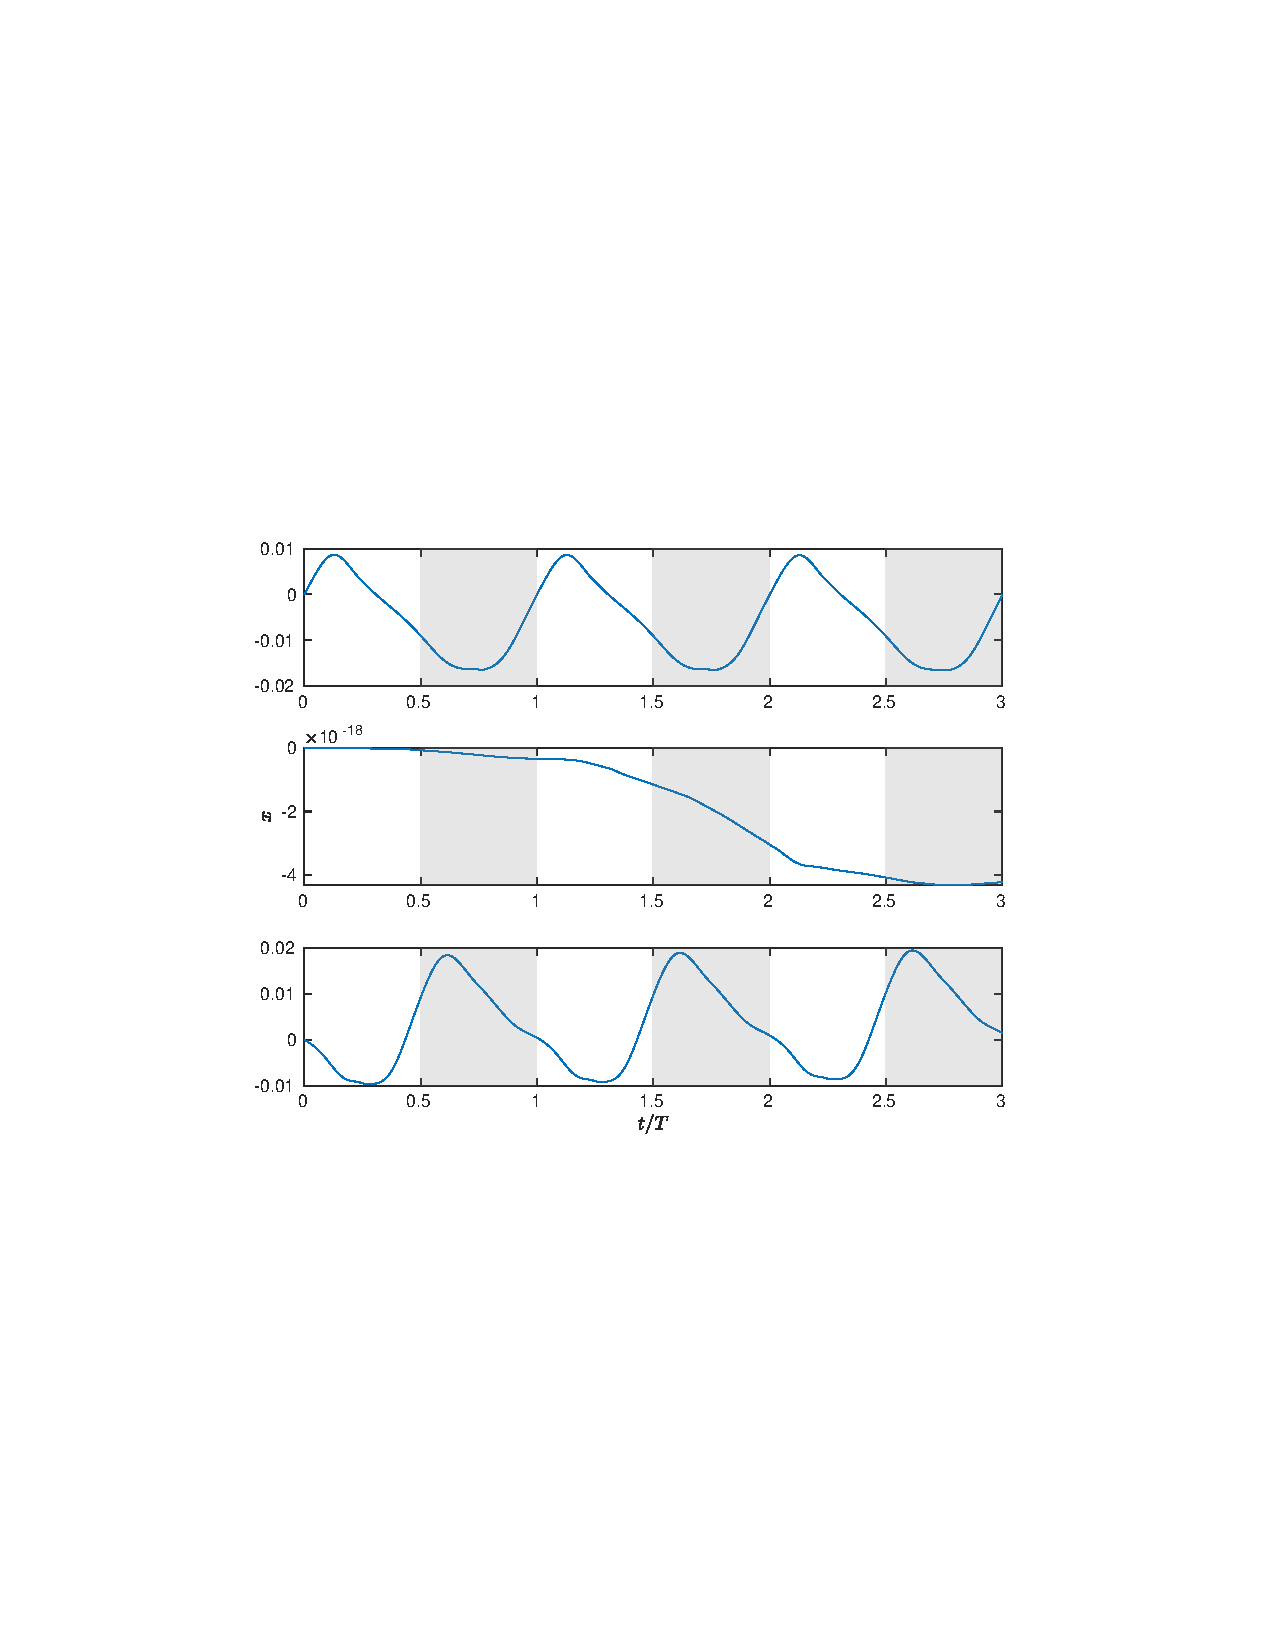
\includegraphics[width=0.75\linewidth]{sim_QS_x_hover_pos.pdf}
	\caption{Position trajectory}
\end{figure}

\begin{figure}[h!]
	\centering
	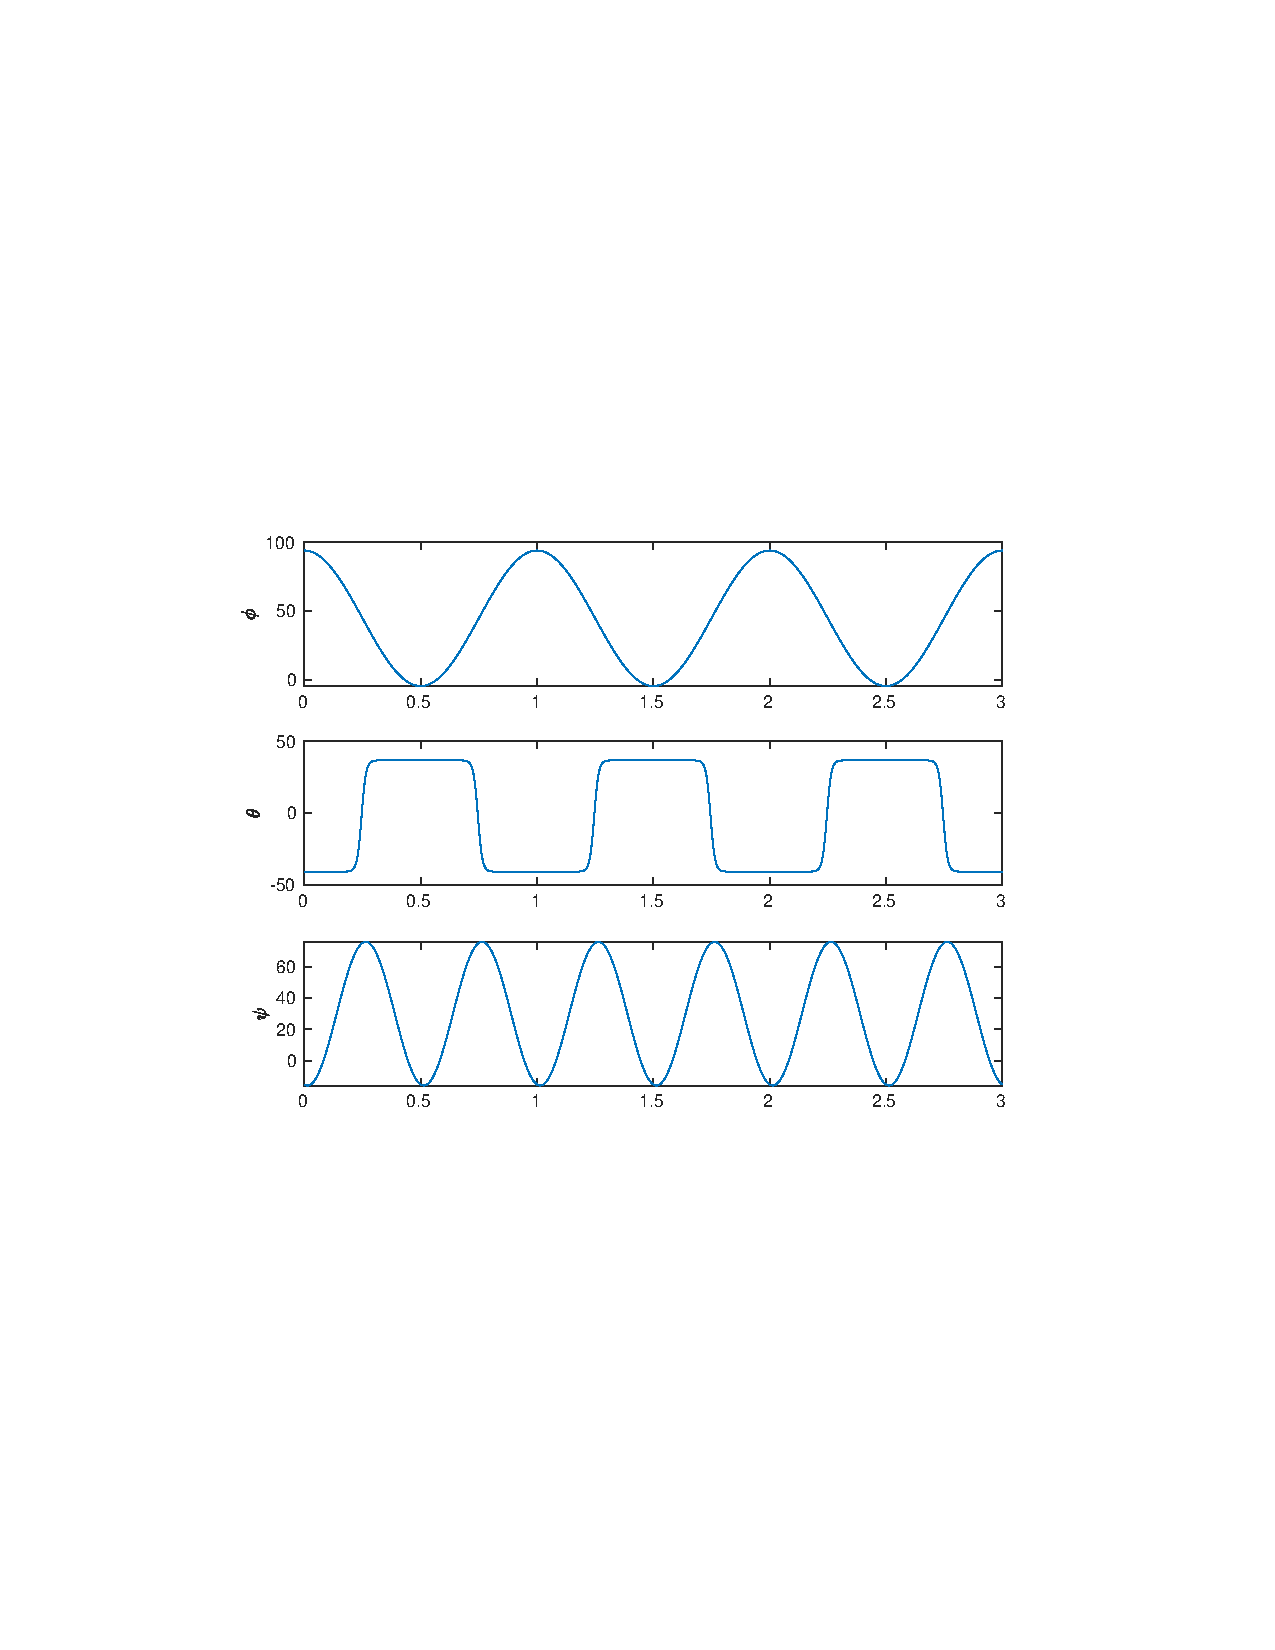
\includegraphics[width=0.75\linewidth]{sim_QS_x_hover_kin.pdf}
	\caption{Euler angle values}
\end{figure}

\end{document}